% Generated by documents/paper/figures/make_rq_appendix.py from the rq01_scaling_predictability README; do not edit.
\clearpage
\section{Scaling predictability}
\label{app:rq01_scaling_predictability}

\begin{rqfinding}
1. \textbf{Accuracy scales log-linearly where it is above chance:} 1165 gated (task, K) fits over 418 benchmark tasks, median R$^2$ 0.88 (IQR 0.77--0.94); per-language BPB 1.00 (106 fits, 50 languages), training loss 0.98--1.00 at every K. (Figure~\ref{fig:app_rq01_scaling_predictability}.)

2. \textbf{The gate decides which benchmarks have a law at all:} 428 of 896 accuracy and BPB tasks are at chance wherever a fit was possible, and 17 of 42 families lose every task, among them Global-PIQA parallel (0/63), Belebele (0/59), INCLUDE (0/36) and Global-MMLU (0/29).

3. \textbf{A letter-answer benchmark's bBPB scales far better once reformulated:} over the eight letter-format families the original's bBPB fits at median R$^2$ 0.81 and its \texttt{rf\_} twin's at 0.98 (530 fits each, 3--4 rungs).
\end{rqfinding}

\paragraph{Question.} Which benchmarks, and which per-language measurements, move with model size in a way a log-linear fit captures, so that a small-model measurement has a trend to extrapolate from at all?

\paragraph{Setup.} Log-linear fits of each task's final score against model size, one series per task and language setting, on the sizes where the task is above chance (at least three); deep baseline-data cells at seed 1904, 90M--1.7B. Each task is one point, the median over its language settings.

\begin{figure}[h]
\centering
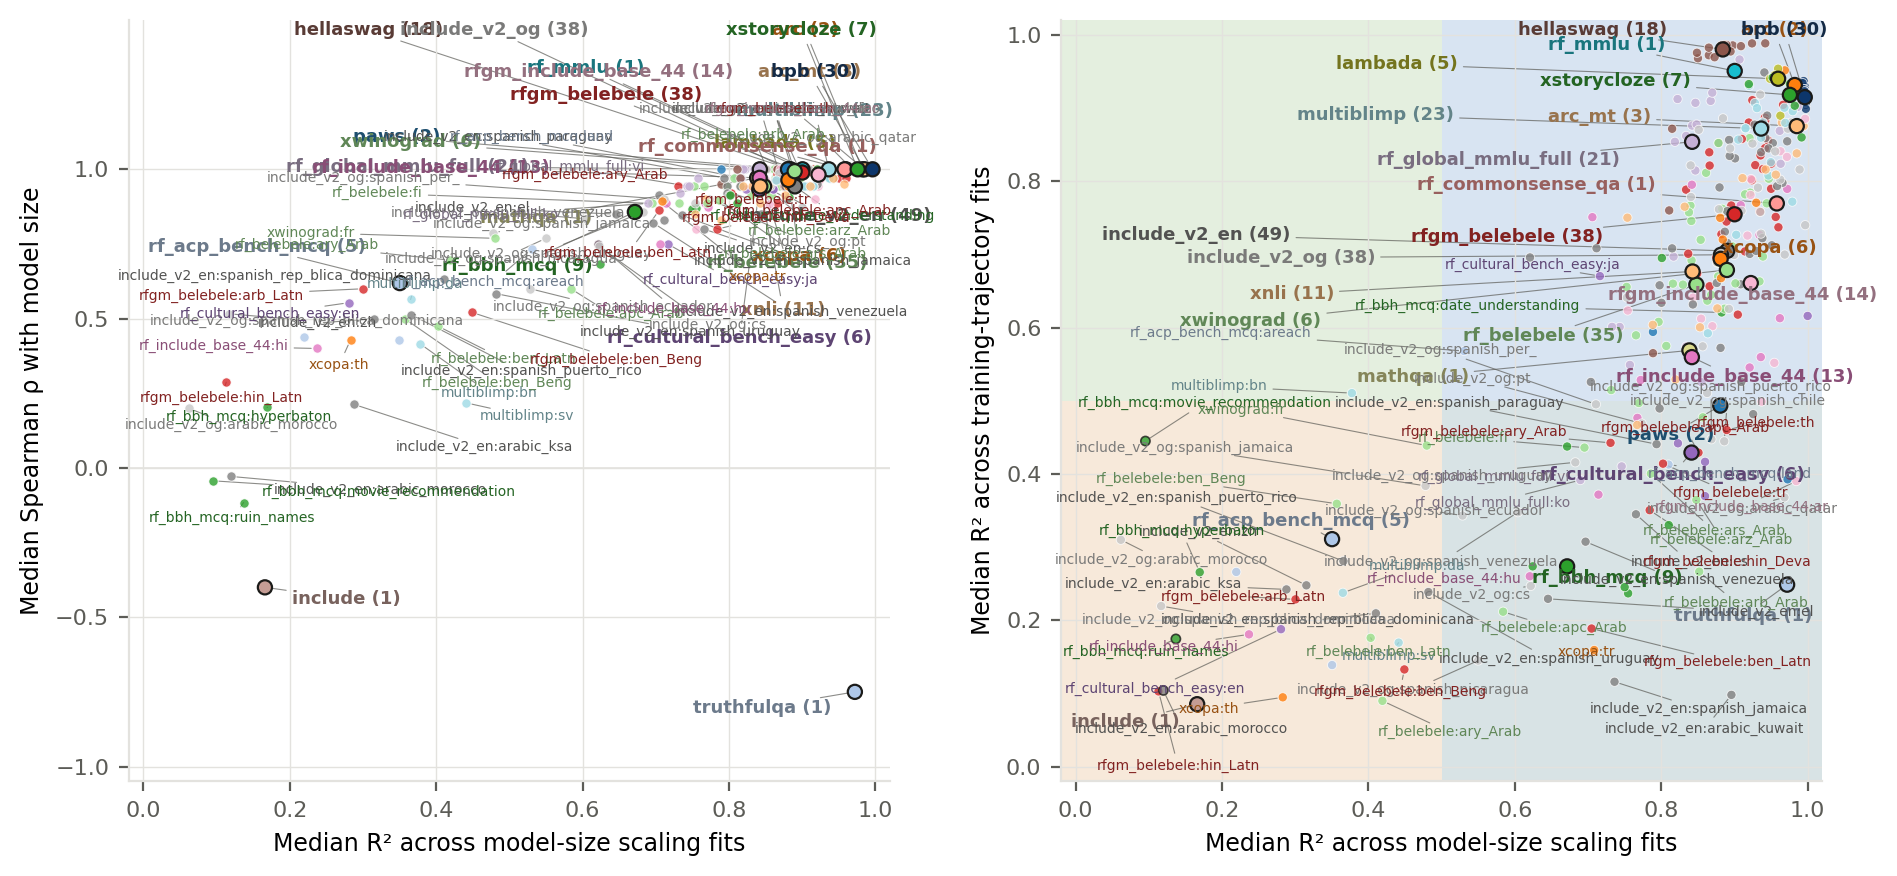
\includegraphics[width=\textwidth]{figures/rq1.png}
% source: src/signal-and-noise/analysis/rq01_scaling_predictability/pretraining/predictivity_seeds/scaling_regimes_outliers_paper.png
\caption{Scaling regimes.}
\label{fig:app_rq01_scaling_predictability}
\end{figure}
